\chapter{Examples}

This chapter describes three examples of how \dfastmi could be used.

\section{Example 1: secondary channel along the Waal}

For this (manually analyzed) case the effect of the secondary channel was analyzed by means of the results of a 1D \sobek model instead of 2D WAQUA or \dflowfm simulation results.
The secondary channel is located along the Waal river at chainage 900-905 km.
The secondary channel was represented in the 1D Rijntakken model as a local lateral extraction of river discharge.
The extraction was 3 \% of the total river discharge up to 4000 m\textsuperscript{3}/s beyond that the discharge increases linearly up to 10 \% at 7000 m\textsuperscript{3}/s and higher discharges.
The effect on the main channel discharge is shown for a number of characteristic cross-sectional profiles in \autoref{Fig7}.
The changes in the \emph{main channel} discharge caused by the secondary channel do not simply follow from the relationship between the secondary channel discharge and the \emph{total} river discharge.
After all, the secondary channel also lowers the water level which introduces a non-linear effect in particular in the lower range of the flood discharges.
As a result the \emph{main channel} discharge does not decrease proportionally to the extra flow area added by the secondary channel (e.g.~at the profile at km 900.5 at Bovenrijn discharges between 7000 and 8000 m\textsuperscript{3}/s).

\begin{figure}
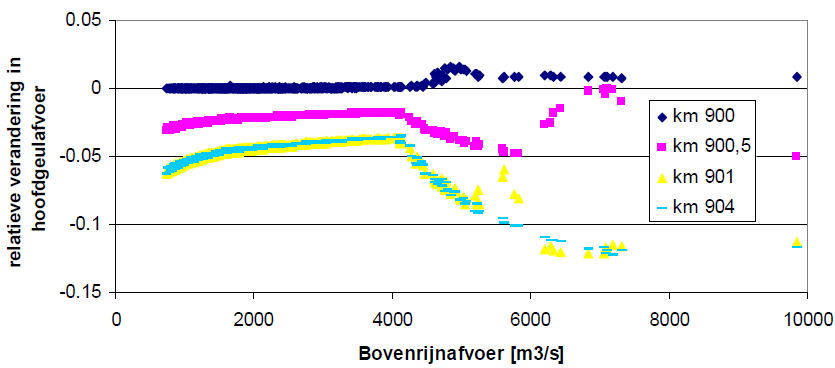
\includegraphics[width=\columnwidth]{figures/Fig7.png}
\caption{Influence of a secondary channel on the main channel discharge of the Waal}
\label{Fig7}
\end{figure}

\subsubsection*{Step 1) Characterize the measure}

The secondary channel removes 3 \% of the total discharge for all discharges below 4000 m\textsuperscript{3}/s in the Bovenrijn.
Above that value the withdrawal increases linearly up to 10 \% at 7000 m\textsuperscript{3}/s.
There is no threshold discharge for the secondary channel: it is active at all discharges.
The secondary channel reaches bankfull at a river discharge of 4000 m\textsuperscript{3}/s.

\subsubsection*{Step 2) Define the discharge blocks}

Because there is no threshold discharge the discharge $Q_1 = 3000$ m\textsuperscript{3}/s is used for the first (low flow) block.
For the second block (transitional discharges) applies that the secondary channel reaches bankfull at 4000 m\textsuperscript{3}/s, so $Q_2 = 4000$ m\textsuperscript{3}/s.
The discharge $Q_3$ of the third block (flood) is in agreement with \autoref{Tab7} equal to 6000 m\textsuperscript{3}/s.
These values can be used to compute the relative duration of each block as

\begin{itemize}
\item $Q_1=3000$ m\textsuperscript{3}/s implies $T_1 = 1-e^{\frac{800-3000}{1280}} = 0.84$
\item $Q_2=4000$ m\textsuperscript{3}/s implies $T_2 = e^{\frac{800-3000}{1280}} - e^{\frac{800-4000}{1280}} = 0.09$
\item $Q_3=6000$ m\textsuperscript{3}/s implies $T_3 = 1-T_1-T_2 = 0.07$
\end{itemize}

\subsubsection*{Step 3) Equilibrium bed level changes}

For each of the three characteristic discharges the equilibrium bed level changes were determined for each relevant cross-sectional profile based on the \sobek results as

\begin{equation}
\Delta z_{b,i,\text{eq}} = -h_o \frac{Q_{\text{main channel},n} - Q_{\text{main channel},o}}{Q_{\text{main channel},o}}
\end{equation}

\Note Usually the results of a 2D model are used for each individual computational point in the main channel.
However, for this application based on \sobek results the total main channel discharge and the average main channel depth were used which thus only verifies the impact along a single stream path.

The resulting equilibrium values are shown in \autoref{Fig8}.

\begin{figure}
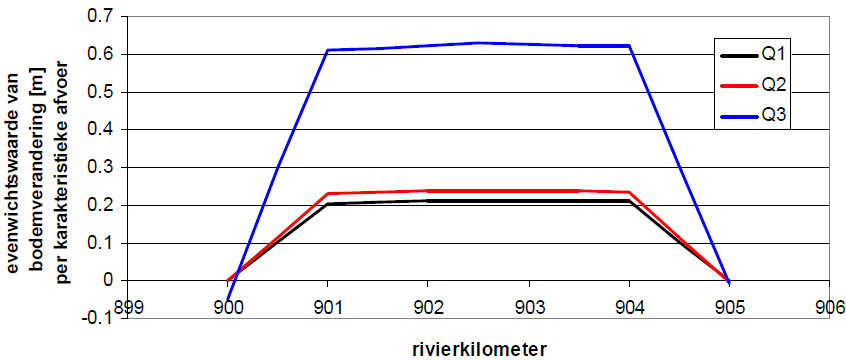
\includegraphics[width=\columnwidth]{figures/Fig8.png}
\caption{Equilibrium bed level changes in the main channel of the Waal at the site of the secondary channel.}
\label{Fig8}
\end{figure}

\subsubsection*{Step 4) Time scales for relaxation}

The main channel width (normal width between groyne heads) at the site of the secondary channel is 260 m.
The bed celerity for low discharges is 900 m/yr; for high discharges this increases to 3650 m/yr.
Consequently, for each block we can compute

\begin{align}
\sigma_1 &= e^{-\frac{w_l}{2B_n}T_1} = e^{-\frac{900}{2 \cdot 260} 0.84} = 0.18 \\
\sigma_2 &= e^{-\frac{w_l}{2B_n}T_2} = e^{-\frac{3650}{2 \cdot 260} 0.09} = 0.73 \\
\sigma_3 &= e^{-\frac{w_l}{2B_n}T_3} = e^{-\frac{3650}{2 \cdot 260} 0.07} = 0.78
\end{align}

\subsubsection*{Step 5) Computation of the characteristic bed level changes}

Based on the equilibrium values determined in step 3 and the relaxation factors of step 4 the characteristic bed level changes can be computed using

\begin{align}
z_{b,1}(0) &= \frac{z_{b,1,\text{eq}} (1-\sigma_1) \sigma_2 \sigma_3 + z_{b,2,\text{eq}} (1-\sigma_2) \sigma_3 + z_{b,3,\text{eq}} (1-\sigma_3)}{(1 - \sigma_1 \sigma_2 \sigma_3} \\
z_{b,2}(0) &= \frac{z_{b,1,\text{eq}} (1-\sigma_1) + z_{b,2,\text{eq}} (1-\sigma_2) \sigma_3 \sigma_1 + z_{b,3,\text{eq}} (1-\sigma_3) \sigma_1}{1 - \sigma_1 \sigma_2 \sigma_3}
\end{align}

To illustrate, the third characteristic bed level change has also been determined by means of
%
\begin{equation}
z_{b,3}(0) = \frac{z_{b,1,\text{eq}} (1-\sigma_1) \sigma_2 + z_{b,2,\text{eq}} (1-\sigma_2) + z_{b,3,\text{eq}} (1-\sigma_3) \sigma_1 \sigma_2}{1 - \sigma_1 \sigma_2 \sigma_3}
\end{equation}

For instance for cross-sectional profile km 901 we obtain $\Delta z_{b,1,\text{eq}} = 0.20$ m; $\Delta z_{b,2,\text{eq}} = 0.23$ m; $\Delta z_{b,3,\text{eq}} = 0.61$ m.
Substitution of these values into the aforementioned equations gives for km 901

\begin{align}
z_{b,1}(0) &= \tfrac{0.20 \cdot (1-0.18) \cdot 0.73 \cdot 0.78 + 0.23 \cdot (1-0.73) \cdot 0.78 + 0.61 \cdot (1-0.78)}{1 - 0.18 \cdot 0.73 \cdot 0.78} = 0.31 \\
z_{b,2}(0) &= \tfrac{0.20 \cdot (1-0.18) + 0.23 \cdot (1-0.73) \cdot 0.78 \cdot 0.18 + 0.61 \cdot (1-0.78) \cdot 0.18}{1 - 0.18 \cdot 0.73 \cdot 0.78} = 0.22 \\
z_{b,3}(0) &= \tfrac{0.20 \cdot (1-0.18) \cdot 0.73 + 0.23 \cdot (1-0.73) + 0.61 \cdot (1-0.78) \cdot 0.18 \cdot 0.73}{1 - 0.18 \cdot 0.73 \cdot 0.78} = 0.22
\end{align}

\subsubsection*{Step 6) Visualizing the results}

The alongstream profile of the characteristic bed level changes is shown together with the results obtained from \sobek in \autoref{Fig9}.
The $z_{b,1}(0)$ value (the characteristic maximum bed level change at the end of the flood period) corresponds in this case well with the bed level change that is not exceeded during 98 \% of the time.
the $z_{b,2}(0)$ value (the characteristic minimum bed level change at the end of the low flow period) corresponds in this case well with the bed level change which is not exceeded during 50 \% of the time.
The $z_{b,3}(0)$ value is in this particular case almost equal to $z_{b,2}(0)$ and it thus exceeds the simulated value that corresponds to the value not exceeded during 2 \% of the time.

\begin{figure}
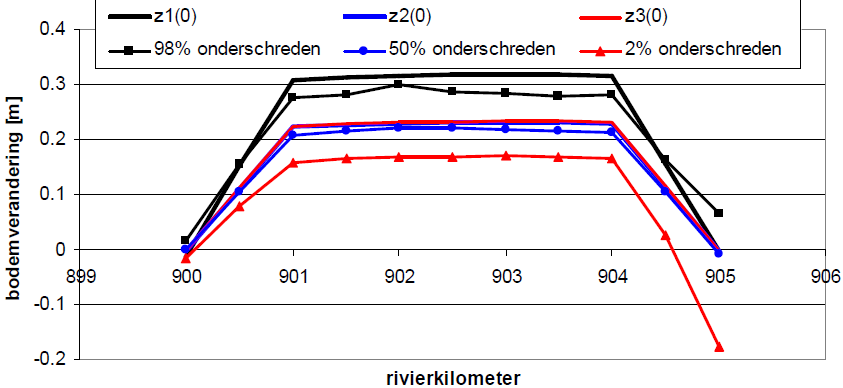
\includegraphics[width=\columnwidth]{figures/Fig9.png}
\caption{Estimated and simulated bed level changes at the secondary channel along the Waal.}
\label{Fig9}
\end{figure}

\section{Example 2: secondary channel along the Lek}

The second case also concerns a secondary channel; however, this time a secondary channel along the Lek between km 930 and km 935.
Also this secondary channel has been schematized as a local lateral extraction of flow from the overall river.
This extraction corresponds again to 3 \% of the total discharge for values up to 4000 m\textsuperscript{3}/s and increases linearly beyond to that 10 \% at 7000 m\textsuperscript{3}/s and higher discharges.
The effect on the main channel discharge is shown for a number of representative cross-sections in \autoref{Fig10}.

\begin{figure}
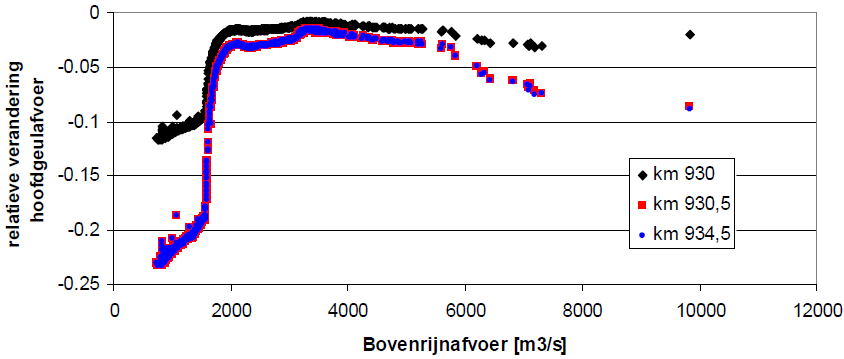
\includegraphics[width=\columnwidth]{figures/Fig10.png}
\caption{Influence of the secondary channel on the main channel discharge for the Lek}
\label{Fig10}
\end{figure}

\subsubsection*{Step 1) Characterize the measure}

The secondary channel extracts 3 \% of the total discharge for Bovenrijn discharges up to 4000 m\textsuperscript{3}/s.
Above that value the withdrawal increases linearly up to 10 \% at 7000 m\textsuperscript{3}/s.
As in the first case there is no threshold discharge since the secondary channel is active for all discharges.
The reaches bankfull at a Bovenrijn discharge of 4000 m\textsuperscript{3}/s.

\subsubsection*{Step 2) Definition of the discharge blocks}

Because there is no threshold discharge the discharge $Q_1 = 1500$ m\textsuperscript{3}/s is used for the first (low flow) block.
For the second block (transitional discharges) applies that the secondary channel reaches bankfull at 4000 m\textsuperscript{3}/s, so $Q_2 = 4000$ m\textsuperscript{3}/s.
The discharge $Q_3$ of the third block (flood) is in agreement with \autoref{Tab7} equal to 6000 m\textsuperscript{3}/s.
These values can be used to compute the relative duration of each block as

\begin{itemize}
\item $Q_1=1500$ m\textsuperscript{3}/s implies $T_1 = 1-e^{\frac{800-1500}{1280}} = 0.42$
\item $Q_2=4000$ m\textsuperscript{3}/s implies $T_2 = e^{\frac{800-1500}{1280}} - e^{\frac{800-4000}{1280}} = 0.50$
\item $Q_3=6000$ m\textsuperscript{3}/s implies $T_3 = 1-T_1-T_2 = 0.08$
\end{itemize}

\subsubsection*{Step 3) Equilibrium bed level changes}

\begin{figure}
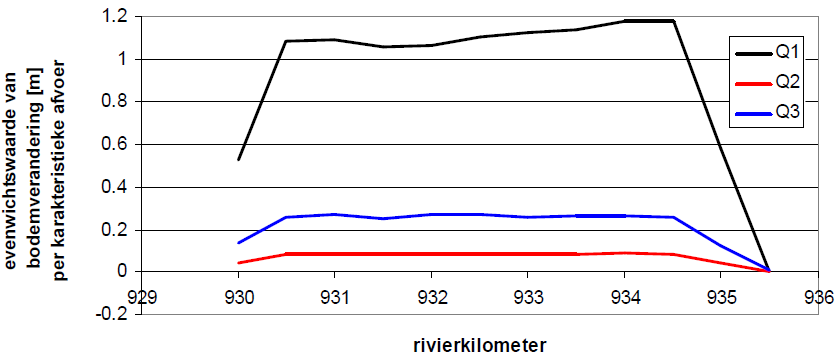
\includegraphics[width=\columnwidth]{figures/Fig11.png}
\caption{Equilibrium bed level changes in the main channel of the Lek at the site of the secondary channel.}
\label{Fig11}
\end{figure}

For each of the three characteristic discharges the equilibrium bed level changes were determined for each relevant cross-sectional profile based on the \sobek results as

\begin{equation}
\Delta z_{b,i,\text{eq}} = -h_o \frac{Q_{\text{main channel},n} - Q_{\text{main channel},o}}{Q_{\text{main channel},o}}
\end{equation}

\Note Usually the results of a 2D model are used for each individual computational point in the main channel.
However, for this application based on \sobek results the total main channel discharge and the average main channel depth were used which thus only verifies the impact along a single stream path.

The resulting equilibrium values are shown in \autoref{Fig11}.

\subsubsection*{Step 4) Time scales for relaxation}

The main channel width (normal width between groyne heads) at the site of the secondary channel is 140 m.
The bed celerity for low discharges is 0 m/yr; for high discharges this increases to 3120 m/yr.
Consequently, for each block we can compute

\begin{align}
\sigma_1 &= e^{-\frac{w_l}{2B_n}T_1} = e^{-\frac{0}{2 \cdot 140} 0.42} = 1.00 \\
\sigma_2 &= e^{-\frac{w_l}{2B_n}T_2} = e^{-\frac{3120}{2 \cdot 140} 0.50} = 0.004 \\
\sigma_3 &= e^{-\frac{w_l}{2B_n}T_3} = e^{-\frac{3120}{2 \cdot 140} 0.08} = 0.40
\end{align}

\subsubsection*{Step 5) Computation of the characteristic bed level changes}

Based on the equilibrium values determined in step 3 and the relaxation factors of step 4 the characteristic bed level changes can be computed.
For instance for cross-sectional profile km 930.5 we obtain $\Delta z_{b,1,\text{eq}} = 1.08$ m; $\Delta z_{b,2,\text{eq}} = 0.08$ m; $\Delta z_{b,3,\text{eq}} = 0.26$ m.
Substitution of these values into the appropriate equations gives for km 930.5

\begin{align}
z_{b,1}(0) &= \tfrac{1.08 \cdot (1-1.00) \cdot 0.004 \cdot 0.40 + 0.08 \cdot (1-0.004) \cdot 0.40 + 0.26 \cdot (1-0.40)}{1 - 1.00 \cdot 0.004 \cdot 0.40} = 0.20 \\
z_{b,2}(0) &= \tfrac{1.08 \cdot (1-1.00) + 0.08 \cdot (1-0.004) \cdot 0.40 \cdot 1.00 + 0.26 \cdot (1-0.40) \cdot 1.00}{1 - 1.00 \cdot 0.004 \cdot 0.40} = 0.20 \\
z_{b,3}(0) &= \tfrac{1.08 \cdot (1-1.00) \cdot 0.004 + 0.08 \cdot (1-0.004) + 0.26 \cdot (1-0.40) \cdot 1.00 \cdot 0.004}{1 - 1.00 \cdot 0.004 \cdot 0.40} = 0.08
\end{align}

\subsubsection*{Step 6) Visualizing the results}

\begin{figure}
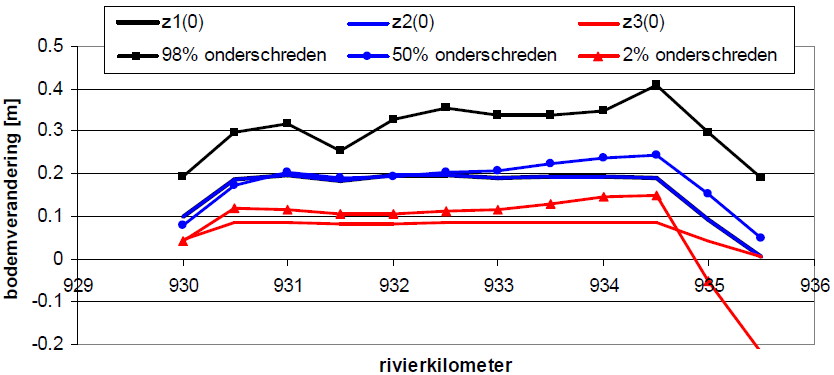
\includegraphics[width=\columnwidth]{figures/Fig12.png}
\caption{Estimated and simulated bed level changes at the secondary channel along the Lek.}
\label{Fig12}
\end{figure}

The alongstream profile of the characteristic bed level changes is shown together with the results obtained from \sobek in \autoref{Fig12}.
The $z_{b,1}(0)$ value (the characteristic maximum bed level change at the end of the flood period) corresponds in this case to the $z_{b,2}(0)$ value (the characteristic minimum bed level change at the end of the low flow period).
Both values correspond in this case well with the bed level change which is not exceeded during 50 \% of the time.
The $z_{b,3}(0)$ value corresponds in this particular case to the value not exceeded during 2 \% of the time.


\section{Example 3: an application to the Maas}

This example shows an analysis that was carried out using the original WAQMORF tool, but results of the latest \dfastmi program are consistent so it's still relevant.
The analysis was based on results obtained using the WAQUA model of "Over de Maas" of \citep{Svasek2007}.
The simulation results were provided by Ed Lemaire (DLB).

The test consisted of the following steps

\begin{enumerate}
\item The tool \dfastmi was used to determine the --- for the morphology --- representative discharges.
This step returned the discharges 1250 m\textsuperscript{3}/s, 1500 m\textsuperscript{3}/s and 2000 m\textsuperscript{3}/s at Borgharen.

\item WAQUA simulations were carried for both the reference situation and situation with the measure implemented.
The water depths and flow velocities were exported using WAQVIEW to the export files supported by \dfastmi.

\item The export files were used as input for a second run of \dfastmi to estimate i) the mean annual bed level change, ii) the maximum bed level change (at the end of the flood season) and iii) the minimum bed level change (at the end of the low flow season)
\end{enumerate}

\begin{figure}
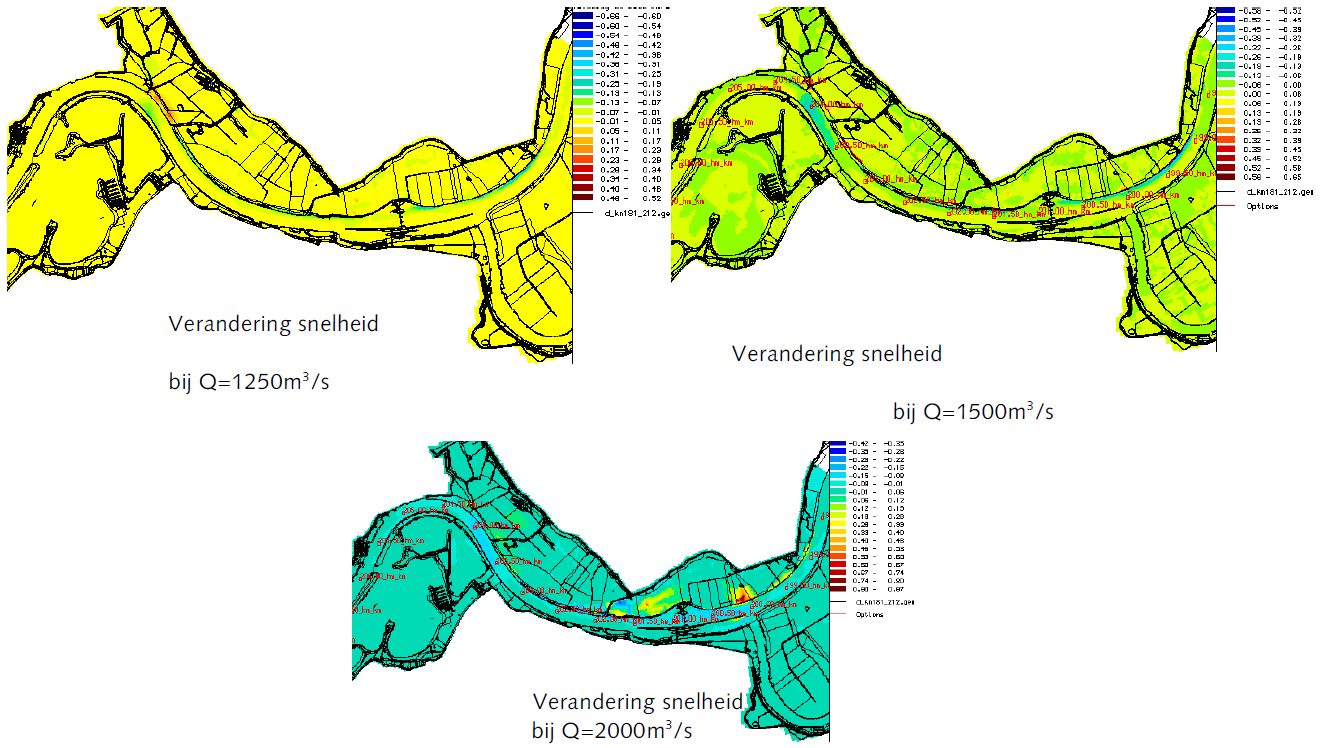
\includegraphics[width=\columnwidth]{figures/Fig13.png}
\caption{Overview of the velocity changes due to the measure}
\label{Fig13}
\end{figure}

The biggest local bed level changes are located in the bend immediately downstream of the measure.
The figures show the mean annual bed level changes in cm for three different critical velocities for the initiation of motion.
This parameter turns out to have little effect in this particular case.
The impact of the plan on river maintenance can be determined based on the available space in the navigation channel.

\begin{figure}
\center
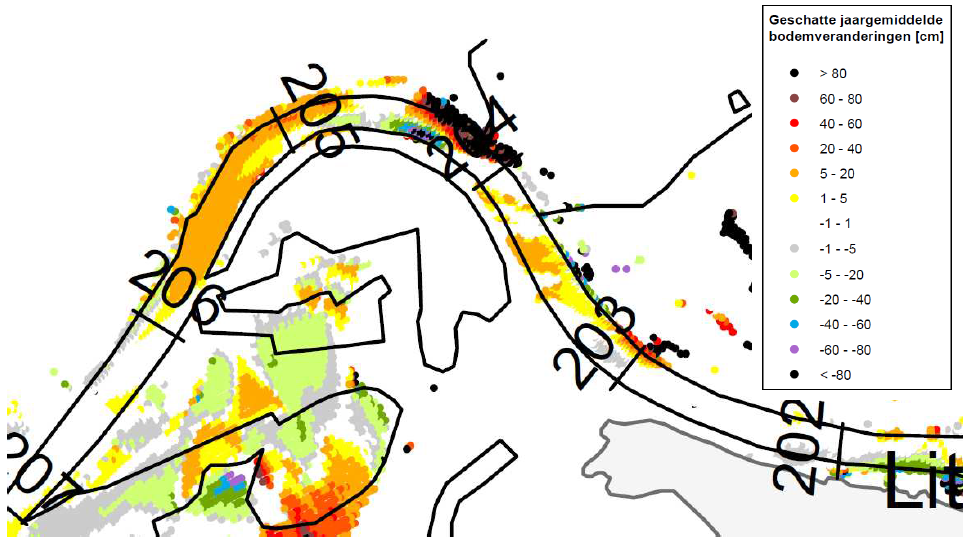
\includegraphics[width=12cm]{figures/Fig14a.png}
\caption{Estimated bed level changes (velocity threshold $u_{crit} = 0.01$ m/s).}
\label{Fig14a}
\end{figure}

\begin{figure}
\center
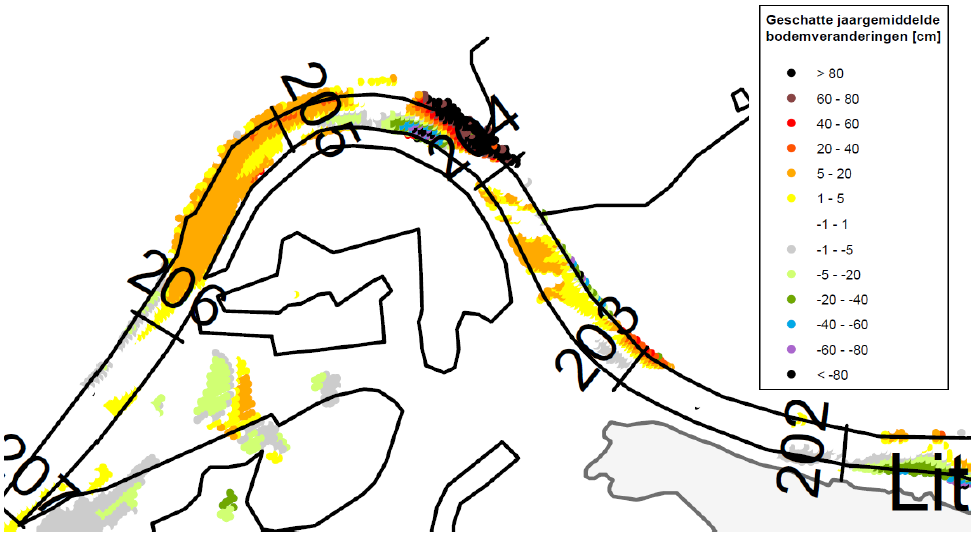
\includegraphics[width=12cm]{figures/Fig14b.png}
\caption{Estimated mean annual bed level changes (velocity threshold $u_{crit} = 0.10$ m/s).}
\label{Fig14b}
\end{figure}

\begin{figure}
\center
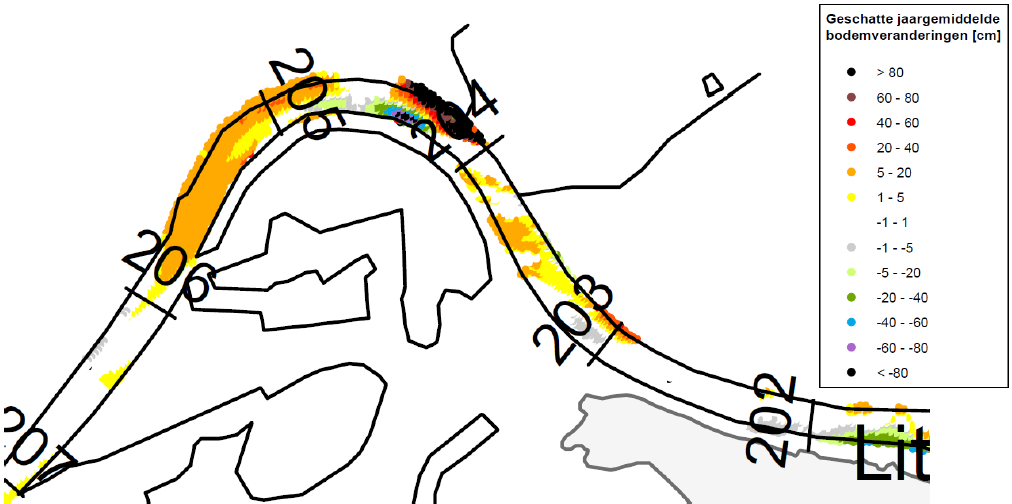
\includegraphics[width=12cm]{figures/Fig14c.png}
\caption{Estimated mean annual bed level changes (velocity threshold $u_{crit} = 0.30$ m/s).}
\label{Fig14c}
\end{figure}
